\begin{lemma}
    Let $\vec{p}_1, \vec{p}_2$ be the orthogonal eigenvectors of the symmetric matrix $\vec{V}$, defined by 
    \begin{align}
        \vec{x}^T\vec{V}\vec{x} + 2\vec{u}^T\vec{x} + f =0
    \end{align}
    
The axes of the conics are given by 
\begin{align}
    \vec{p}_1^T\brak{\vec{x}-\vec{c}} &= 0
    \\
    \vec{p}_2^T\brak{\vec{x}-\vec{c}} &= 0
\end{align}
where,$\vec{c}$ is the vertex of conic.
\end{lemma}

\begin{proof}
According to the principal axis theorem,
\begin{enumerate}
    \item Each eigen vector of $\vec{V}$ is parallel to either the major axis or minor axis.
    \item Axes pass through the vertex $\vec{c}$ of the conic.
\end{enumerate}

\end{proof}
{\em Examples: }
\begin{enumerate}    
    \item Parabola
    \begin{align}
    y^2-4x+2y+4 = 0
    \end{align}
    
    Here,
    \begin{align}
    \vec{V} &= \myvec{0 & 0 \\ 0 & 1} \\
    \vec{u} &= \myvec{-2 \\ 1} \\
    f &= 4
    \end{align}
    Now,
    \begin{align}
    \myvec{-4 & 1 \\ 0 & 0 \\ 0 & 1}\vec{c} &= \myvec{-4 \\ 0 \\ -1}
    \\
    \implies \vec{c} &= \myvec{\frac{3}{4} \\ -1}
    \end{align}
    So,
    \begin{align}
    \brak{\vec{x}-\vec{c}} &= \myvec{x-\frac{3}{4} \\  y+1}
    \end{align}
    
    Now,
    \begin{align}
        \mydet{\vec{V}-\lambda\vec{I}} &= 0 \\
        \implies \mydet{-\lambda & 0 \\ 0 & 1-\lambda} &= 0 \\
        \implies \lambda_1 =0,\lambda_2 &= 1
    \end{align}
    
    For $\lambda_1=0$,
    \begin{align}
        \vec{V}-\lambda_1\vec{I} &= \myvec{0 & 0 \\ 0 & 1} \\
        \implies \vec{p_1} &= \myvec{1 \\ 0}
    \end{align}
    
    Similarly for $\lambda_2=1$,
    \begin{align}
        \vec{p_2} &=\myvec{0 \\ 1}
    \end{align}
    
    
    \begin{figure}[!ht]
    \centering
    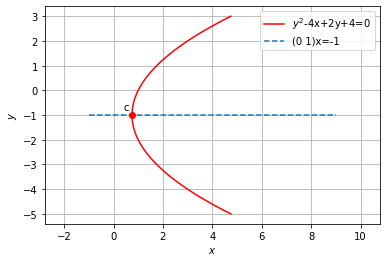
\includegraphics[width=\columnwidth]{app/2/Figures/ChallengeProblem5_2.png}
    \caption{$y^2$-4x+2y+4=0}
    \label{quadforms/app/2/ex2}	
    \end{figure}
   
    $\because \lambda_2>\lambda_1$ \\
    Hence,the axis using $\vec{p_2}$ is given by
    \begin{align}
        \vec{p_2}^T\brak{\vec{x}-\vec{c}} &= 0 \\
        \implies \myvec{0 & 1}\myvec{x-\frac{3}{4} \\ y+1} &= 0 \\
        \implies y+1 &= 0 \\
        \implies \boxed{\myvec{0 & 1}\vec{x} =-1}
    \end{align}
    \item Parabola
    \begin{align}
        y^2 &= 8x
        \\
        \implies y^2-8x &= 0
    \end{align}
    
    Here,
    \begin{align}
    \vec{V} &= \myvec{0 & 0 \\ 0 & 1} \\
    \vec{u} &= \myvec{-4 \\ 0} \\
    f &= 0
    \end{align}
    Now,
    \begin{align}
    \myvec{-8 & 1 \\ 0 & 0 \\ 0 & 1}\vec{c} &= \myvec{0 \\ 0 \\ 0}
    \\
    \implies \vec{c} &= \myvec{0 \\ 0}
    \end{align}
    
    So,
    \begin{align}
    \brak{\vec{x}-\vec{c}} &= \myvec{x \\ y}
    \end{align}
    
    Now,
    \begin{align}
        \mydet{\vec{V}-\lambda\vec{I}} &= 0 \\
        \implies \mydet{-\lambda & 0 \\ 0 & 1-\lambda} &= 0 \\
        \implies \lambda_1 =0,\lambda_2 &= 1
    \end{align}
    
    For $\lambda_1=0$,
    \begin{align}
        \vec{V}-\lambda_1\vec{I} &= \myvec{0 & 0 \\ 0 & 1} \\
        \implies \vec{p_1} &= \myvec{1 \\ 0}
    \end{align}
    
    Similarly for $\lambda_2=1$,
    \begin{align}
        \vec{p_2} &=\myvec{0 \\ 1}
    \end{align}
    $\because \lambda_2>\lambda_1$ \\
    Hence,the axis using $\vec{p_2}$ is given by
    \begin{align}
        \vec{p_2}^T\brak{\vec{x}-\vec{c}} &= 0 \\
        \implies \myvec{0 & 1}\myvec{x \\ y} &= 0 \\
        \implies y &= 0\\
        \implies \boxed{\myvec{0 & 1}\vec{x} =0}
    \end{align}
    
    
    \begin{figure}[!ht]
    \centering
    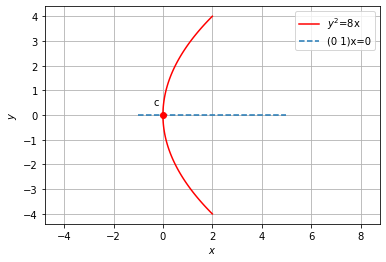
\includegraphics[width=\columnwidth]{app/2/Figures/ChallengeProblem5_3.png}
    \caption{$y^2$=8x}
    \label{quadforms/app/2/ex3}	
    \end{figure}
    
    \item Ellipse
    \begin{align}
        x^2+xy+y^2 &= 100
    \end{align}
    
    Here,
    \begin{align}
    \vec{V} &= \myvec{1 & \frac{1}{2} \\ \frac{1}{2} & 1} \\
    \vec{u} &= \myvec{0 \\ 0} \\
    f &= -100
    \end{align}
    Now,
    \begin{align}
    \vec{c} &= \vec{V}^{-1}\vec{u}\\
    \implies \vec{c} &= \myvec{0 \\ 0}
    \end{align}
    So,
    \begin{align}
    \brak{\vec{x}-\vec{c}} &= \myvec{x \\ y}
    \end{align}
    
    Now,
    \begin{align}
        \mydet{\vec{V}-\lambda\vec{I}} &= 0 \\
        \implies \mydet{1-\lambda & \frac{1}{2} \\ \frac{1}{2} & 1-\lambda} &= 0 \\
        \implies \lambda^2-2\lambda+\frac{3}{4} &= 0 \\
        \implies \lambda_1 =\frac{1}{2},\lambda_2 &= \frac{3}{2}
    \end{align}
    
    For $\lambda_1=\frac{1}{2}$,
    \begin{align}
        \vec{V}-\lambda_1\vec{I} &= \myvec{\frac{1}{2} & \frac{1}{2} \\ \frac{1}{2} & \frac{1}{2}} \\
        \implies \vec{p_1} &= \frac{1}{\sqrt{2}}\myvec{-1 \\ 1}
    \end{align}
    
    Similarly for $\lambda_2=\frac{3}{2}$,
    \begin{align}
        \vec{p_2} &= \frac{1}{\sqrt{2}}\myvec{1 \\ 1}
    \end{align}
    
    $\because \lambda_2>\lambda_1$ \\
    Hence,the major axis using $\vec{p_2}$ is given by
    \begin{align}
        \vec{p_2}^T\brak{\vec{x}-\vec{c}} &= 0 \\
        \implies \frac{1}{\sqrt{2}}\myvec{1 & 1}\myvec{x \\ y} &= 0 \\
        \implies x+y &= 0 \\
        \implies \boxed{\myvec{1 & 1}\vec{x} =0}
    \end{align}
    
    and the minor axis using $\vec{p_1}$ is given by
    \begin{align}
        \vec{p_1}^T\brak{\vec{x}-\vec{c}} &= 0 \\
        \implies \frac{1}{\sqrt{2}}\myvec{-1 & 1}\myvec{x \\ y} &= 0 \\
        \implies -x+y &= 0 \\
        \implies \boxed{\myvec{-1 & 1}\vec{x} =0}
    \end{align}
    
    
    \begin{figure}[!ht]
    \centering
    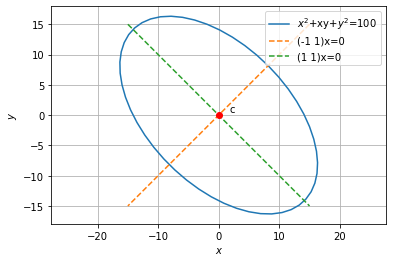
\includegraphics[width=\columnwidth]{app/2/Figures/ChallengeProblem5_4.png}
    \caption{$x^2$+xy+$y^2$=100}
    \label{quadforms/app/2/ex4}	
    \end{figure}
    
    \item Hyperbola
    \begin{align}
        xy-3y+2 &= 0
    \end{align}
    
    Here,
    \begin{align}
    \vec{V} &= \frac{1}{2}\myvec{0 & 1 \\ 1 & 0} \\
    \vec{u} &= \frac{-3}{2}\myvec{0 \\ 1} \\
    f &= 2
    \end{align}
    Now,
    \begin{align}
    \vec{c} &= \vec{V}^{-1}\vec{u}\\
    \implies \vec{c} &= \myvec{3 \\ 0}
    \end{align}
    So,
    \begin{align}
    \brak{\vec{x}-\vec{c}} &= \myvec{x-3 \\ y}
    \end{align}
    Now,
    \begin{align}
        \mydet{\vec{V}-\lambda\vec{I}} &= 0 \\
        \implies \mydet{-\lambda & \frac{1}{2} \\ \frac{1}{2} & -\lambda} &= 0 \\
        \implies \lambda^2-\frac{1}{4} &= 0 \\
        \implies \lambda_1 =\frac{-1}{2},\lambda_2 &= \frac{1}{2}
    \end{align}
    
    For $\lambda_1=\frac{-1}{2}$,
    \begin{align}
        \vec{V}-\lambda_1\vec{I} &= \myvec{\frac{1}{2} & \frac{1}{2} \\ \frac{1}{2} & \frac{1}{2}} \\
        \implies \vec{p_1} &= \frac{1}{\sqrt{2}}\myvec{-1 \\ 1}
    \end{align}
    
    Similarly for $\lambda_2=\frac{1}{2}$,
    \begin{align}
        \vec{p_2} &= \frac{1}{\sqrt{2}}\myvec{1 \\ 1}
    \end{align}
    
    
    \begin{figure}[!ht]
    \centering
    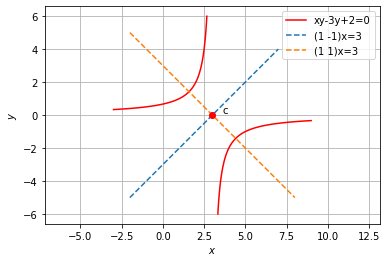
\includegraphics[width=\columnwidth]{app/2/Figures/ChallengeProblem5_5.png}
    \caption{xy-3y+2=0}
    \label{quadforms/app/2/ex5}	
    \end{figure}
    
    $\because \lambda_2>\lambda_1$ \\
    Hence,the major axis using $\vec{p_2}$ is given by
    \begin{align}
        \vec{p_2}^T\brak{\vec{x}-\vec{c}} &= 0 \\
        \implies \frac{1}{\sqrt{2}}\myvec{1 & 1}\myvec{x-3 \\ y} &= 0 \\
        \implies x+y &= 3 \\
        \implies \boxed{\myvec{1 & 1}\vec{x} =3}
    \end{align}
    
    and the minor axis using $\vec{p_1}$ is given by
    \begin{align}
        \vec{p_1}^T\brak{\vec{x}-\vec{c}} &= 0 \\
        \implies \frac{1}{\sqrt{2}}\myvec{-1 & 1}\myvec{x-3 \\ y} &= 0 \\
        \implies x-y &= 3 \\
        \implies \boxed{\myvec{1 & -1}\vec{x} =3}
    \end{align}
    
\end{enumerate}



